%Template by Mark Jervelund - D1 - 2015 - mjerv15@student.sdu.dk

\documentclass[a4paper,10pt,titlepage]{report}

\usepackage[utf8]{inputenc}
\usepackage[T1]{fontenc}
\usepackage[english]{babel}
\usepackage{amssymb}
\usepackage{amsmath}
\usepackage{amsthm}
\usepackage{graphicx}
\usepackage{fancyhdr}
\usepackage{lastpage}
\usepackage{listings}
\usepackage{algorithm}
\usepackage{algpseudocode}
\usepackage[document]{ragged2e}
\usepackage[margin=1in]{geometry}
\usepackage{color}
\usepackage{datenumber}
\usepackage{venndiagram}
\usepackage{chngcntr}
\setdatetoday
\addtocounter{datenumber}{0} %date for dilierry standard is today
\setdatebynumber{\thedatenumber}
\date{}
\setcounter{secnumdepth}{0}
\pagestyle{fancy}
\fancyhf{}

\newcommand{\Z}{\mathbb{Z}}
\lhead{Database Management Systems (DM556))}
\rhead{Mark Jervelund (Mjerv15) Troels Petersen (trpet15)}
\rfoot{Page  \thepage \, of \pageref{LastPage}}
\counterwithin*{equation}{section}

\lstset{
  numbers=left,
  stepnumber=5,    
  firstnumber=1,
  numberfirstline=true
  frame=single,
  breaklines=true,
  postbreak=\raisebox{0ex}[0ex][0ex]{\ensuremath{\color{red}\hookrightarrow\space}}
}

\begin{document}
\begin{titlepage}
\centering
    \vspace*{9\baselineskip}
    \huge
    \bfseries
    Project 1\\
    
    \normalfont 
	\huge    
    Database Management Systems (DM556)  \\[4\baselineskip]
    \normalfont
	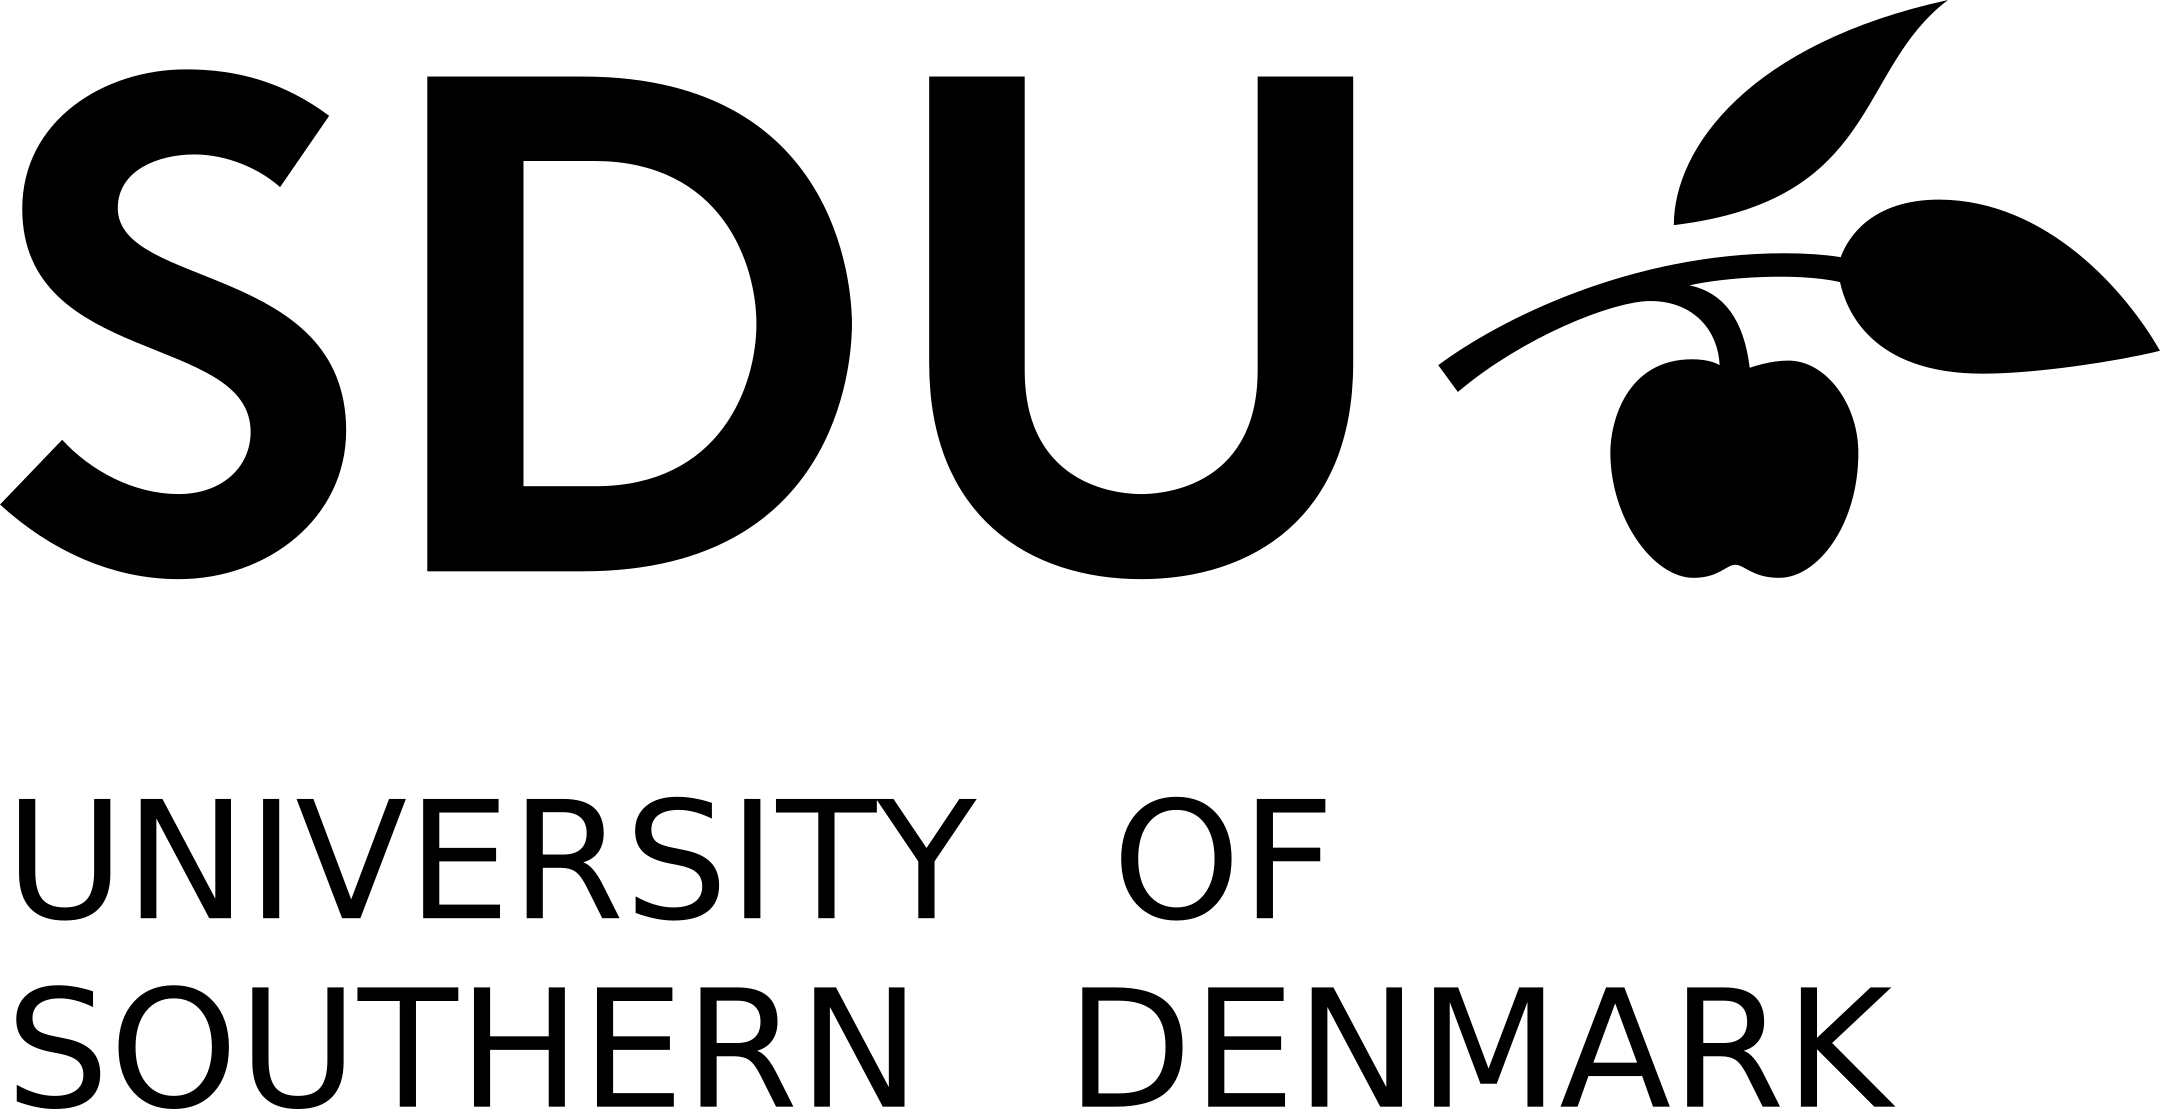
\includegraphics[scale=1.5]{SDU_Logo}
    \vfill\ 
    \vspace{5mm}
    IMADA \\
Mark Jervelund (Mjerv15) Troels Petersen (trpet15)
    \textbf{\datedate}  \bf{at 16-20} \\[2\baselineskip]
\end{titlepage}
%\renewcommand{\thepage}{\roman{page}}% Roman numerals for page counter
%\tableofcontents

%\newpage
\setcounter{page}{1}
\renewcommand{\thepage}{\arabic{page}}

\lstset{language=Java}          % Set your language (you can change the language for each code-block optionally)
\section{Overall Status}
The overall status of of project is that we 
\section{Division of Labor}
\subsection{Specification}


\subsection{Design}

 

\subsection{Implementation}

\subsection{Testing}

\subsection{Conclusion}
\end{document}
